\chapter{Satellite Design}
\label{chap:SatDesign}
To simulate the ADCS of the satellite the sensors and actuators that will be used for the CubeSat must be decided. This decision is based on the current trend and implementation of CubeSat as well as what is required of this mission of pointing the payload towards the Earth during eclipse and being sun-following otherwise.

The trend from $1990$ to $2015$ of what sensors and actuators small satellites implement for the ADCS system is provided in Figure~\ref{fig:SensorOccurances} and Figure~\ref{fig:ActuatorOccurances} \cite{JansevanVuuren2015}. A study conducted by \cite{Jacklin2019} provides examples of $2$ partially failed missions that are due to sensor failure. One of which is ascribe to magnetometer faults and one towards that of the sun sensor. Another total mission failure is due to the failure of both the magnetometer and sun sensor. There is however no example of partial or total mission failure due to any other sensor failure. It should however be noted that the sun sensor and magnetometer are more frequently implemented in the period of \cite{Jacklin2019} research as shown in Figure~\ref{fig:SensorOccurances}. Since most satellites implement a magnetometer and a sun sensor, these two sensors are used in the simulation environment of this thesis and practical anomalies are modelled for these two sensors.

The horizon sensor, although it is only utilized by $10\%$ of small satellites ADCS operations has an interesting anomaly~\cite{wessels2018infrared}. The anomaly of the horizon sensor is the moon on the earth horizon and influencing the algorithm for calculating the centre of the Earth. This anomaly will occur often and is unavoidable through the CubeSat design. This anomaly will therefore will be modelled and the influence of the anomaly on the sensor measurement will be discussed.

\begin{figure}
\centering
	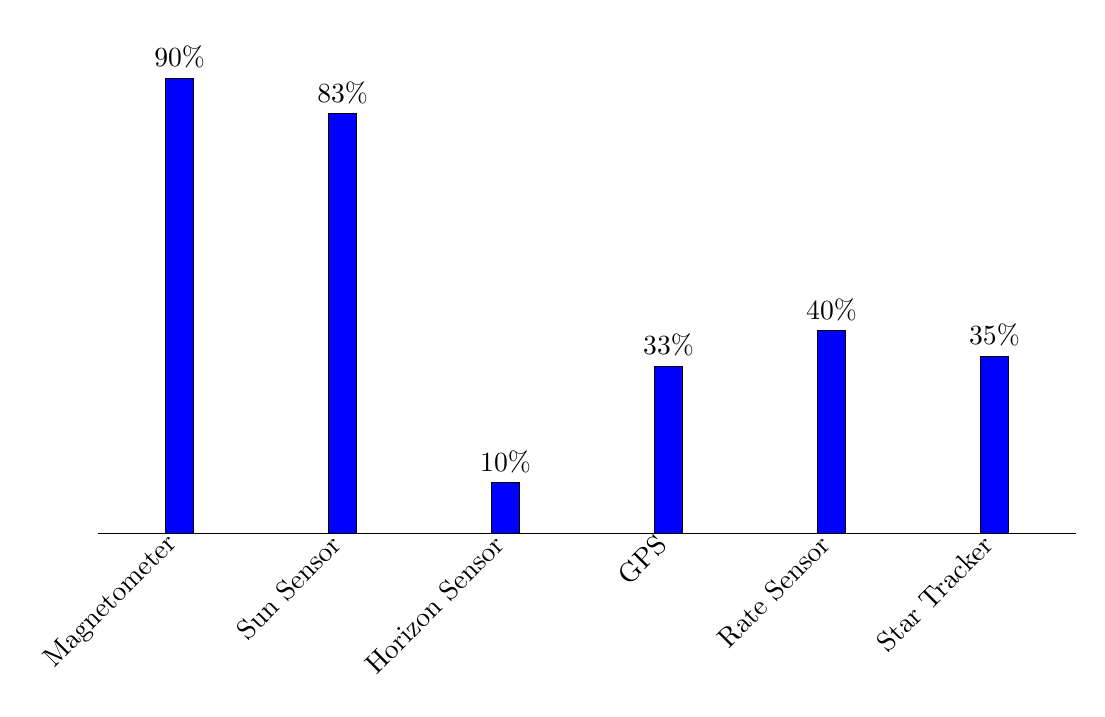
\begin{tikzpicture}
		\begin{axis}[height=8cm, width=14cm,
		symbolic x coords={Magnetometer,Sun Sensor,Horizon Sensor,GPS,Rate Sensor,Star Tracker},
		xtick=data,
		ymin=0, ymax=100,
		x tick label style={rotate=45,anchor=east},
		axis y line*=left,
		axis x line*=bottom,
		y axis line style={draw=none},
		grid=none,
		nodes near coords=\pgfmathprintnumber{\pgfplotspointmeta}\%,
		tick style={draw=none},
		ytick = \empty
		]
		
		\addplot[ybar,fill=blue] coordinates {
			(Magnetometer,90)
			(Sun Sensor,83)
			(Horizon Sensor,10)
			(GPS,33)
			(Rate Sensor,40)
			(Star Tracker,35)
		};
		\end{axis}
	\end{tikzpicture}
\caption{The percentage occurances of different ADCS sensors on small satellites}
\label{fig:SensorOccurances}
\end{figure}

The percentage of ADCS systems that utilizes a variety of actuators is visualised in Figure~\ref{fig:ActuatorOccurances}. It is evident Figure~\ref{fig:ActuatorOccurances} that the two actuators that is utilized the most is the magnetorquers and reaction wheels. Therefore these two actuators are implemented for the the control output of the ADCS. However since the focus of this thesis is to test various methods for robust estimation and the reaction wheels will have a significant influence on the estimation, whereas the magnetorquers will only be implemented for momentum dumping. An anomaly for reaction wheels will therefore be discussed, but the magnetorquers will be assumed to perform perfectly during all operations.

\begin{figure}
	\centering
	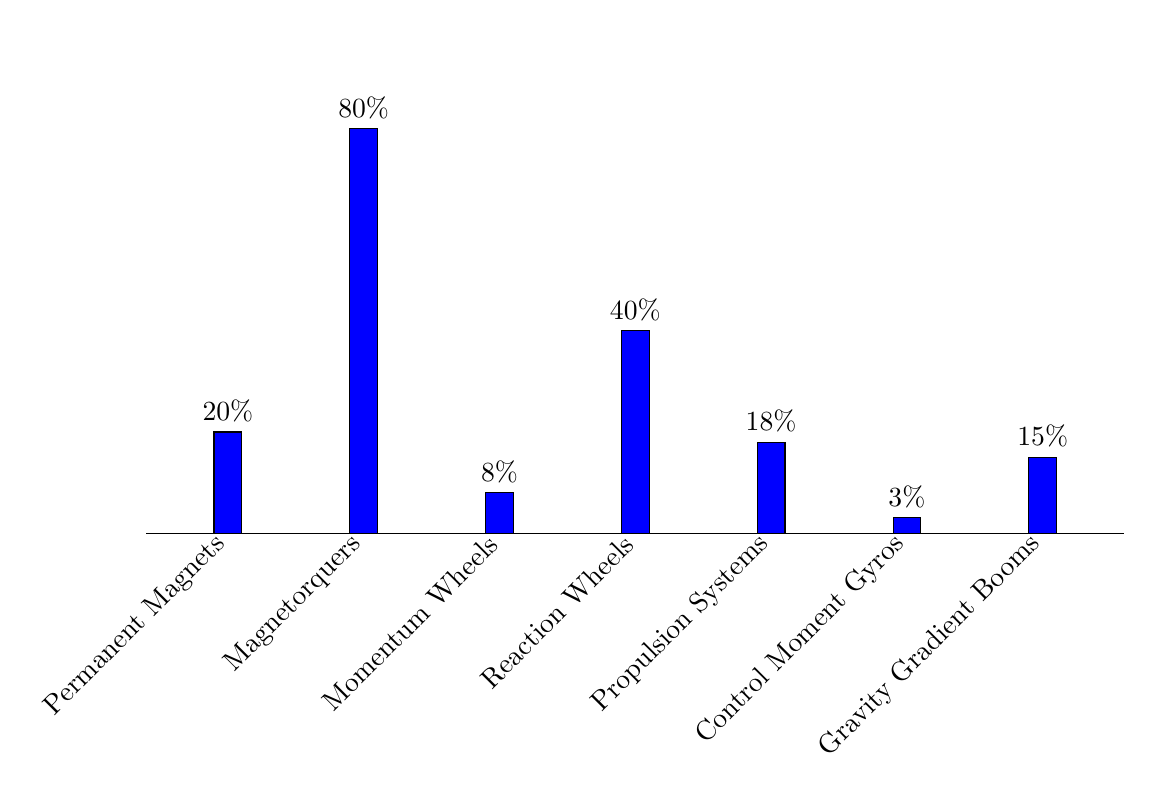
\begin{tikzpicture}
		\begin{axis}[height=8cm, width=14cm,
		symbolic x coords={Permanent Magnets,Magnetorquers,Momentum Wheels,Reaction Wheels,Propulsion Systems,Control Moment Gyros,Gravity Gradient Booms},
		xtick=data,
		ymin=0, ymax=100,
		x tick label style={rotate=45,anchor=east},
		axis y line*=left,
		axis x line*=bottom,
		y axis line style={draw=none},
		grid=none,
		nodes near coords=\pgfmathprintnumber{\pgfplotspointmeta}\%,
		tick style={draw=none},
		ytick = \empty
		]
		
		\addplot[ybar,fill=blue] coordinates {
			(Permanent Magnets,20)
			(Magnetorquers,80)
			(Momentum Wheels,8)
			(Reaction Wheels,40)
			(Propulsion Systems,18)
			(Control Moment Gyros,3)
			(Gravity Gradient Booms,15)
		};
		\end{axis}
	\end{tikzpicture}
	\caption{The percentage occurances of different ADCS actuators on small satellites}
	\label{fig:ActuatorOccurances}
\end{figure}

\section{CubeSat}
To ensure accurate modelling and simulation of the satellite orbit as well as anomaly modelling a outer design of the CubeSat is required. The elements that required specific dimensions for the dynamics and kinematics is the solar panels and the satellite body. The sun sensor also requires specific dimensions for the sun reflection anomaly discussed in Section~\ref{section:Reflection} and the dimensions of the sun sensor are from the Sputnix CubeSat sun sensor model. The summary of these dimensions is given in Table~\ref{Table:Dimensions}.

\begin{table}[h!t!b]
	\centering
	\caption{\label{Table:Dimensions}Physical dimensions of simulated CubeSat}
	\begin{tabular}{c c c c}
		\hline\hline
		Dimensions & Satellite Body & Solar Panels & Sun Sensor \\ \hline
		$\bar{\mathbf{x}}_\mathcal{B}$          & $0.3$ m                    & $0.3$ m                       & $0.028$ m                   \\
		$\bar{\mathbf{y}}_\mathcal{B}$          & $0.3$ m                    & $0.3$ m                       & $0.023$ m                   \\
		$\bar{\mathbf{z}}_\mathcal{B}$          & $0.4$ m                    & $0.002$ m                     & N/A                     \\
		\hline\hline
	\end{tabular}
\end{table}

An entire solar panel is denoted as the surface area of ABCD as shown in Figure~\ref{fig:CubeSatDesign}. This will be referenced for the sun reflection anomaly as well as the magnetic moment disturbance anomaly. The coordinate frames and the background thereof will be discussed in Section~\ref{section:CoordinateFrames}.

\begin{figure}[h!t!b]
	\centering
	\def\svgwidth{14cm}
	\import{Figures/}{CubeSatDesign.pdf_tex}
	\caption{The modelled satellite, with solar panels.}
	\label{fig:CubeSatDesign}
\end{figure}

\section{Sensors}
Infra-red horizon sensor ~\cite{wessels2018infrared}. 
Sun sensor Sputnix CubeSat sun sensor
\begin{table}[h!t!b]
	\centering
	\caption{\label{Table:SensorNoise}Standard deviation for each sensor}
	\begin{tabular}{c c c c}
		\hline\hline
		\textbf{Sensor} & Standard deviation as percentage ($\sigma$) \\ \hline
		Magnetometer & 0.75 \\
		Earth Sensor & 0.14 \\
		Sun Sensor & 0.055 \\
		\hline\hline
	\end{tabular}
\end{table}
\textbf{TODO: The sensors that is implemented as well as the noise variation on each sensor and the placement thereof}.

\section{Actuators}
, RW-0.06 from Sinclair Interplanetary, $U_d = 2.08e^{-9}$ and $U_s = 2.08e^{-7}$
\textbf{TODO: Ud and Us and other parameters as well as reaction wheel orientation and inertia}.